\section{Koord Software Stack}
\label{sec:software}

\subsection{Runtime system}



To run a $\lgname$ program (hardware or simulation), the user has to provide a configuration file, with
\begin{inparaenum}
    \item the number of agents,
    \item in case of simulation, the initial positions of the agents and the length of the simulation and
    \item in case of hardware deployment their IP addresses,
    and the localization system.
\end{inparaenum}

\subsection{Key environment assumptions}


\subsubsection{Periodic event execution semantics}


\subsubsection{Shared variable implementation over message passing}


\subsubsection{Known set of participants}
\subsubsection{Portability and heterogeneity}


\subsection{Simulator}
\subsubsection{gazebo environment}
\subsubsection{car model}
\subsubsection{lidar}
\subsubsection{positioning}
\subsubsection{sampled sensing}
\subsubsection{synchronization issues}

\subsection{The Distributed Mapping Problem}
In this section, we introduce the distributed mapping problem. Informally, the problem requires a set of robots to collaboratively mark the position of static \emph{obstacles} within a given area $D$, which any robot should avoid while moving in $D$.The key difference between distributed SLAM and this application is that we assume that the robots know their \emph{global coordinates} within the area of deployment. They are only attempting to map the static obstacles within this area. We currently assume that the only sensors available for sensing obstacles are LIDAR based, and the robots are constrained to move in a 2-D space.


\subsubsection{Preliminaries}
\label{sec:prelims}
We first set up the terminology and assumptions to discuss our approach to this problem.

The mapping problem is defined over a (\emph{bounded}) domain $D$, a bounded rectangle in $\mathbb{R}^2$ given by $[a_1,a_2]\times [b_1,b_2]$.

\begin{definition}
    A \emph{quantization} of a bounded domain $D$ is defined as a mapping $\qfunc:D \mapsto \qdom$ where $\qdom = \left\{q_{ij}\right\}_{i\in [1..n_x], j\in [1..n_y]}$ such that every $q_{ij}$ corresponds to a \emph{grid rectangle} $[x_i, x_{i+1}] \times [y_j, y_{j+1}]$.
\end{definition}

We assume the existence of a \emph{ground truth} function $\world : D\mapsto \left\{0,1\right\}$, where $\forall \Vec{x} \in D$, $$\world(\Vec{x}) = \begin{cases}
                                                                                                                                                                        1\ \mbox{if there is an obstacle at }\Vec{x}\\
                                                                                                                                                                        0\ \mbox{otherwise}
\end{cases}
$$


\begin{definition}
    Given a quantized domain $Q$, a \emph{\qdfunc} over $Q$ is any function $F$ with the signature $Q^\prime \mapsto \left\{0,1\right\}$, where $F$ is only defined on $Q^\prime \subset Q$, and it maps each $q_i \in Q^\prime$ to either 0 or 1.
\end{definition}


Given any quantization $Q$ of the domain $D$ given by $\qfunc:D\mapsto Q$, the corresponding \qdfunc
$\world_Q : Q \mapsto \left\{0,1\right\}$ is defined as follows,  $$\world_Q(q) = \begin{cases}
                                                                                      1\ \Leftrightarrow \exists \Vec{x}\in D, \qfunc(\Vec{x}) = q \wedge \world(\Vec{x}) = 1 \\
                                                                                      0\ \mbox{otherwise}
\end{cases}
$$


\rg{Consider that there is a set of ground robots $[N]$, which are tasked with creating a mapping of static obstacles in $Q$ collaboratively by constructing local mappings based on sensed information.}


\begin{definition}
    The \emph{sensing area} of a robot $i$ at position $\pos(i)\in D$ is defined by $\sensarea_i: Q \mapsto 2^{Q}$, such that there is a \qdfunc $\rmap : \sensarea_i \mapsto \left\{0,1\right\}$, where $$\forall q \in \sensarea_i(\qfunc(\pos_i)), \rmap(q) = \world_Q(q).$$
    Given a robot $i \in [N]$, $\sensarea_i$ may depend both on the position of the robot as well as the range of the LIDAR scanner.
\end{definition}



Let $\map_i:Q\mapsto \left\{-1,0\right\}$ denote a \qdfunc \emph{local} to robot $i$, which we see as a \emph{software state} for a given robot $i$.  % $\map_i(q) = 1$ indicates that according to robot $i$, there is an obstacle in $q$, $\map_i(q) = 0$ indicates that according to robot $i$, $q$ is unoccupied, and $\map_i(q) = -1$ indicates that robot $i$ doesn't have information about $q$.



We assume that given $\Vec{x} \in q, \forall \Vec{x^\prime} \in q, \sensarea(\Vec{x}) \subseteq \sensarea(\Vec{x^\prime})$. We can now state the 2-d distributed mapping problem, $\mapprob$ as follows. \begin{quote}
{\em Given a quantization, $\qfunc:D\mapsto Q$ of a 2-d domain $D\subset \mathbb{R}^2$, a ground truth function $\world:D \mapsto \left\{0,1\right\}$, a set of robots $[N]$ , for each robot $i \in [N]$ construct an \emph{occupancy map} which is a $\qdfunc$, $\map_i: Q_i \mapsto \left\{1,0\right\}$, $Q_i\subseteq Q$.
}
\end{quote}

% \rg{We can \emph{combine} the elements of the set of \emph{local maps}, $\{\map_i\}_{i\in [N]}$ to form a \emph{global} occupancy mapping. }

Having stated the problem, we now define the notion of soundness of a proposed occupancy map.
\begin{definition}
    \label{soundness}
    For a robot $i$, a proposed occupancy mapping over $Q_i\subset Q$, given by $\map_i: Q_i \mapsto \left\{-1,0\right\}$ is \emph{sound} if :
    \begin{itemize}
        \item $\map_i(q) = v \Rightarrow \world_Q(q)  = v$
        \item $\forall v \in \left\{0,1\right\}\world_Q(q) = v \Rightarrow \map(q) = v \vee q\notin Q_i$
    \end{itemize}
\end{definition}


These two statements collectively state that given a proposed occupancy map, \emph{any grid rectangle in the domain of the occupancy map marked as 0 is indeed obstacle free, and if it is marked as 1 then there is indeed an obstacle at least partially in it.}

A vacuously correct (sound) solution to $\mapprob$ given $D, \qfunc$ and $\world_Q$ is $\forall i \in [N]$, $$\map_i : Q_i \mapsto \left\{0,1\right\}, Q_i = \phi$$ To allow for more interesting solutions than the one stated above, we assume that we are given that initially, each robot $i\in[N]$ starts at a grid rectangle with no obstacle, the sensed area of each robot $i$ is non empty, and there is at least one obstacle free rectangle within the sensed area of each robot:
$\forall i \in [N], \world_Q(q^0_i) = 0 \wedge \exists q \in \sensarea(q^0_i), \world_Q(q) = 0 $ and
where $q^0_i = \qfunc(\pos_0(i))$, and $\pos_0(i)$ denotes the initial position of robot $i$.


\begin{definition}
    Given  $i , j \in [N]$, two proposed occupancy mappings $\map_i: Q_i\mapsto\left\{0,1\right\}$ and $\map_j: Q_j\mapsto \left\{0,1\right\}$, are consistent only if $\forall q \in Q_i \cup Q_j, \map_i(q) = \map_j(q)$.
\end{definition}

    Given $\map_i$, $\map_j$, and $q\in Q_i \cup Q_j$ , let $\map_i(q) = 1$, and $\map_j(q) = 0$. Suppose $\map_i$ is sound, then $\world_Q(q) = 1$, which implies $\map_j$ is not sound. By the same argument, if $\map_j$ is sound, $\map_i$ is not. It can be seen that a set of proposed mappings $\left\{\map_i\right\}_{i\in [N]}$, can only be sound if they are pairwise consistent.

We assume that if robot $i$ is at position $\pos(i)$, and it detects an obstacle in $q \in \sensarea(\qfunc(\pos(i)))$, then $q$ does contain an obstacle, otherwise it does not. The point of this presentation isn't dealing with the issue of potentially false positives while identifying an obstacle. A robot partially constructs a grid occupancy function by assigning values to the grid rectangles in its \emph{sensed} area.


%\begin{lemma}
%    \label{ext}
%    Suppose robot $i$ is at $\pos(i)\in D$, and $\exists(q^\prime)\in \sensarea(\pos(i))$,
%    s.t $\map_i(q) = -1$. Consider a mapping, $\map^\prime_i:Q \mapsto \left\{-1,0,1\right\}$
%    such that, $\forall q\in Q \setminus \sensarea(\pos(i)), map^\prime_i(q) = map_i(q)$
%    and $\forall q \in \sensarea(\pos(i)), \map^\prime_i(q) = \world_Q(q)$.
%    Then, $\map^\prime_i(q)$ is sound if $\map_i$ is sound.
%\end{lemma}
%
%The proof for this is straightforward and follows from the definition of $\map^\prime_i$ combined with \defn{soundness}.
%
%Recall from the definition of the sensing area of a robot $i$ at $\pos(i)$, that it can reliably compute the ground truth mapping $\world_Q$ for all $q \in \sensarea(\pos(i))$. This lemma essentially states that given a sound occupancy mapping $\map_i$, it can be used to compute to another \emph{sound} occupancy mapping $\map^\prime_i$ by setting the values of $\map^\prime_i(\sensarea(\pos(i)))$ to the ground truth function.
%
%\begin{definition}
% We say that $\Vec{x_n}\in D$ is \emph{reachable} from $\Vec{x_0}$ if there is a \emph{path} $p = \Vec{x_0},\Vec{x_1}, \Vec{x_2},\ldots, \Vec{x_n}$ , such that
%\begin{itemize}
%\item $\forall i \in [0..n],\world_Q(\qfunc{\Vec{x_i}}) = 0$
%\item a robot can move from $\Vec{x_i}$ to $\Vec{x_{i+1}}$ for $i \in [0..n]$, while staying within $\qfunc(\Vec{x_i}) \cup \qfunc(\Vec{x_{i+1}})$.
%\end{itemize}
%\end{definition}
%
%A grid rectangle $q\in Q$ is reachable in general, if $\exists \Vec{x}\in D, q = \qfunc(\Vec{x})$ such that $\Vec{x}$ is reachable from either \begin{inparaenum} [(a)]\item the initial position of a robot, or \item another reachable point $\Vec{x^\prime}\in D$. We denote the reachability of a grid rectangle using a predicate $\mathit{Reach} : Q \mapsto \left\{\mathit{True}, \mathit{False}\right\}$, where $\mathit{Reach}(q) = \mathit{True}$ if its reachable,  $\mathit{False}$ otherwise.
%\end{inparaenum}
%
%\begin{definition}
%    Given a sound occupancy mapping $\map_i$, the \emph{frontier} of $\map_i$, denoted by $\ff(\map_i)$ is defined as follows:
%    $$ \left\{ q\in Q \mid Reach(q) \wedge \exists q \in \sensarea(\Vec{x}), \map_i(q) = -1\right\} $$
%\end{definition}
%
%Given a sound occupancy mapping $\map_i$, another sound mapping $\map_i^\prime$ can be constructed as shown in \lem{ext}. Taken in conjunction with our assumption on the initial positions of each robot, this leads to a strategy for computing sound occupancy mapping functions. Further, given a set of sound mappings $\left\{\map_i\right\}_{i\in[N]}$, we can construct a sound mapping $\map$ from them as follows :
%
%\begin{lemma}
%    Given a set of sound mappings $\left\{\map_i\right\}_{i\in[N]}$, the mapping described by $\map: Q \mapsto \left\{-1,0,1\right\}$ such that $\map(q) = \mathit{Max}_{i\in[N]}\left\{\map_i(q)\right\}$ is also sound.
%\end{lemma}
%
%\begin{proof}
%    If $\map(q) = 1$, $\exists i\in [N]$, s.t $\map_i(q) = 1$. By \lem{comptbl}, $\forall j \in [N], j\neq i \Rightarrow \map_j(q) = 1\vee \map_j(q) = -1$. Since $\map_i$ is sound, $\map(q) = \world_Q(q)$. The case for $\map(q) = 0$ is also similar. Therefore, $\map(q) = 0\vee \map(q) = 1\Rightarrow \map(q) = \world_Q(q)$. Otherwise, by definition, $\map(q) = -1$, which together with the previous statement, implies that $\map$ is sound.
%\end{proof}
%
%
%
%\subsubsection{Approach}
%
%
%\begin{figure}[!htbp]
%    \centering
%    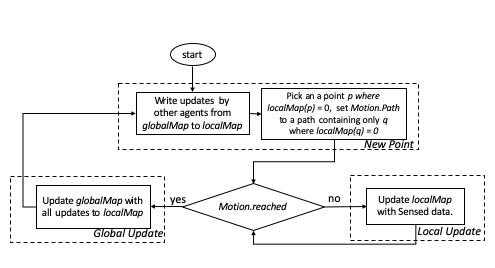
\includegraphics[width=\linewidth]{figs/map_flowchart.png}
%    \caption{Flowchart for a simple solution to 2D distributed mapping problem\vspace{-2mm}}
%    \label{fig:flowmap}
%\end{figure}
%
%
%
%We discuss now discuss how our algorithm implemented $\lgname$ shown in \reffig{mapapp} tackles $\mapprob$. \reffig{flowmap} shows a simple idea for solving this problem for each robot:
%
%The variable $\lmap$ refers to the current mapping $\map_i$ constructed by each robot $i$ using the algorithm. The function $\mathit{MaxExp}$ informally, determines whether there is a grid rectangle in the frontier of the current $\map_i$ . If not, the robot first updates its $\lmap$ from $\gmap$, which is used for sharing the currently computed occupancy maps by all agents so far. The robot then picks a new point in a rectangle known to be unoccupied in its $\lmap$ and follows a path ($\mathit{Motion.Path}$) moving only over grid rectangles known to be unoccupied by its $\lmap$. While the robot hasn't reached the target rectangle, it keeps updating its $\lmap$ with sensed data (occupied and unoccupied rectangles). When it reaches the target, it updates the $\gmap$ from its $\lmap$.
%
%
%

\subsubsection{External (Library) Functions}

% restriction of the world function for sensing. accuracy of sensor statement.
% domain of mapping function for which value is 0 or 1.
% make compatibility a definition instead of lemma.